% Result-integrated manuscript. Sealed v6/v7 and coverage-v1 artifacts are unchanged.
\documentclass[10pt,twocolumn,letterpaper]{article}
\usepackage[review]{cvpr}
% Minimal empirical-study preamble; no historical model macros or number registry.
\usepackage[T1]{fontenc}
\usepackage{times}
\usepackage{amsmath,amssymb}
\usepackage{booktabs}
\usepackage{graphicx}
\usepackage{multirow}
\usepackage{xcolor}
\usepackage{microtype}
\usepackage{enumitem}
\usepackage{placeins}

\definecolor{cvprblue}{rgb}{0.21,0.49,0.74}
\usepackage[pagebackref,breaklinks,colorlinks,allcolors=cvprblue]{hyperref}
\def\paperID{*****}\def\confName{CVPR}\def\confYear{2027}
% Complete analyses validated; this is not a submission-readiness certificate.
\def\ReadoutV6AssetsComplete{1}

\newcommand{\CovFCDY}{-0.332 [-0.436, -0.235]}
\newcommand{\CovFCDE}{+0.916 [+0.755, +1.078]}
\newcommand{\CovFCI}{-1.248 [-1.366, -1.138]}
\newcommand{\CovFCLoneGap}{+0.138 [+0.053, +0.223]}
\newcommand{\CovFCFullGap}{-1.110 [-1.279, -0.951]}
\newcommand{\CovGRDY}{-0.154 [-0.223, -0.083]}
\newcommand{\CovGRDE}{+1.043 [+0.917, +1.169]}
\newcommand{\CovGRI}{-1.197 [-1.306, -1.088]}
\newcommand{\CovGRLoneGap}{-0.157 [-0.259, -0.056]}
\newcommand{\CovGRFullGap}{-1.355 [-1.521, -1.187]}
\newcommand{\CovFullDY}{-0.157 [-0.222, -0.091]}
\newcommand{\CovFullDE}{+1.026 [+0.907, +1.141]}
\newcommand{\CovFullI}{-1.183 [-1.281, -1.081]}
\newcommand{\CovFullLoneGap}{-0.134 [-0.229, -0.039]}
\newcommand{\CovFullFullGap}{-1.316 [-1.463, -1.161]}

\title{Confidence for Which Prediction?\\
Supervision Coverage Shapes Grounding Reliability}
\author{Anonymous submission}
\begin{document}\maketitle
\begin{abstract}
A grounding confidence score must distinguish correct boxes from both
mislocalizations and absent targets. Does supervising that complete success
event suffice? We study matched confidence heads while fixing every output
box of two grounders. Correct-output labels improve correct-versus-wrong
ranking but need not reduce complete-output risk; reading the selected query
does not resolve this tradeoff. A fixed-budget coverage intervention reveals
a more consequential distinction. Expanding positive supervision from L1 to
all difficulty levels lowers correct-output-head AUGRC by 0.332 points on
FineCops, yet raises existence-head risk by 0.916 points, reversing target
preference. Three-state decomposition explains the improvement as better
correct-box/no-target ordering bought at a cost to correct/wrong-box ordering,
not a uniform recovery of correctness. The frozen correct-output head also
improves gRefCOCO risk by 0.154 points. These findings connect confidence
supervision to its training population and show why better existence detection
alone cannot establish more reliable grounding outputs.
\end{abstract}

\begin{figure*}[t]
\centering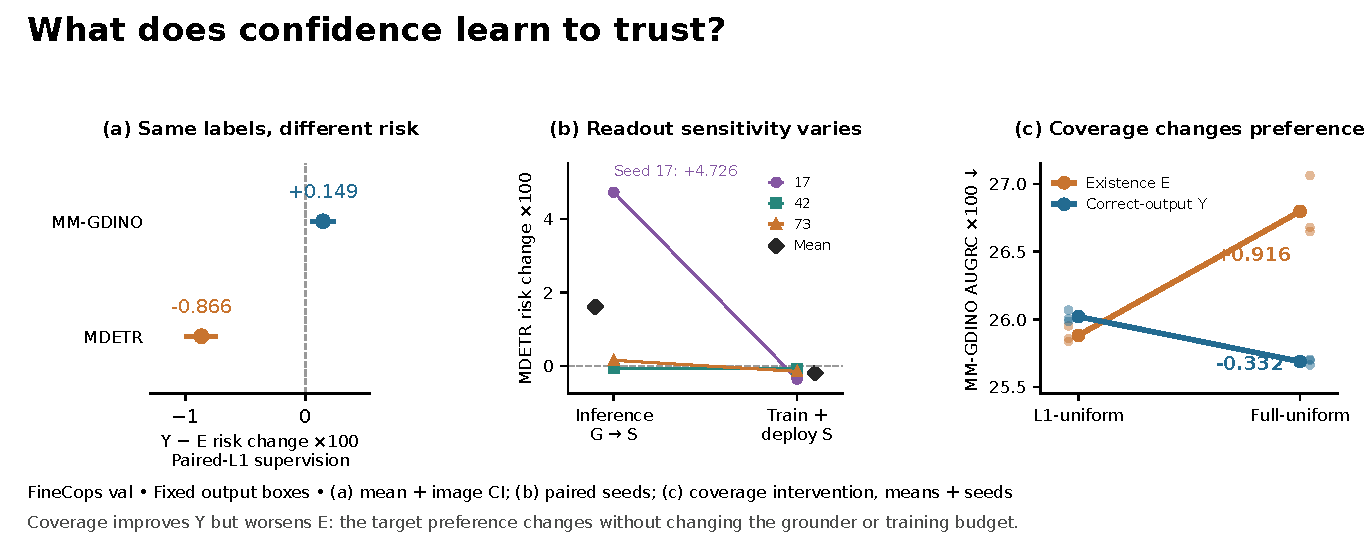
\includegraphics[width=\textwidth]{generated/coverage_v8_r2/figure1_study.pdf}
\caption{\textbf{The training population changes what confidence learns to trust.}
All panels use FineCops validation and fixed Native boxes. (a) Under paired-L1
supervision, changing existence labels (E) to correct-output labels (Y) has
opposite complete-risk effects on two grounders. (b) MDETR inference-only
readout switching is seed-sensitive: seed 17 drives the large mean. Lines show
paired seeds and diamonds their means, not image-bootstrap uncertainty.
(c) A matched coverage intervention on MM-GDINO reduces Y risk but increases
E risk; lines join means and small dots show seeds. Training budget and
readout stay fixed. AUGRC is multiplied by 100; lower is better. Only (a)
shows image-bootstrap intervals, conditional on the three trained heads.}
\label{fig:study}
\end{figure*}

\section{Introduction}
A visual grounding system can return a plausible box for the wrong object,
or for an object that the expression does not identify at all. These are
different failures of the same output decision. Generalized grounding makes
both observable by allowing expressions with no referent
\cite{he2023grec,liu2023gres,liu2024finecops}. A useful confidence score
must retain correct localizations ahead of both failure types.

The apparent solution is to supervise exactly this event: the referent
exists \emph{and} the returned box is correct. An accurate estimate of its
conditional probability would optimally order successes at fixed coverage
under equal failure costs. But a supervision label does not by itself give
such an estimate. The head learns from a particular population of requests,
and the evidence available to its score can differ from the evidence selecting
the output box. We ask: \emph{how do the supervision event and the positive
training population together shape the reliability of a fixed grounder?}

We make this question experimentally separable from localization improvement.
For each of two frozen grounders, every confidence route returns exactly the
same Native box. Matched heads differ only in whether a present-but-wrong
request is labelled valid or unsuccessful. Under a commonly used pairing
construction, positive head supervision reaches only L1 parents of edited
negative expressions. On FineCops, correct-output supervision improves
correct/wrong-box ranking for both grounders, but improves complete risk
only for MDETR. A score can therefore become better at one relevant
comparison without making the overall output decision more reliable.

Two controlled tests sharpen this observation. First, reading the query
that actually supplies the output box does not remove MM-GDINO's disadvantage.
Second, we vary which positives receive supervision, keeping the head,
negative requests, update budget and readout fixed. Expanding from uniformly
sampled L1 positives to the complete positive set \emph{reverses the
preferred supervision target} on FineCops. The Y head improves by 0.332
AUGRC points, while the E head worsens by 0.916. Both directions occur in
all three seeds and persist in frozen transfer to gRefCOCO. This is not
merely a larger gap between two methods: the absolute responses of both
heads identify what produced the reversal.

The explanation lies in the comparisons a complete output score must make.
Let C be a correct box, W a wrong box for an existing referent, and N a
no-target request. Expanding supervision improves Y's C/N ordering, especially
for positives outside the original difficulty coverage, but reduces its C/W
ordering. The first benefit outweighs the second cost at the observed mixture.
For E, the C/W deterioration is much larger: existence AUROC improves even
as complete risk worsens. Thus broader supervision is consequential, but it
does not simply repair every notion of correctness.

Our contribution is a controlled empirical finding about grounding confidence:
\emph{the effect of the supervision event depends on the positive population
used to learn it}. A matched coverage intervention establishes this dependence;
readout controls test a natural alternative explanation; and three-state
analysis connects the observed ranking changes to risk and its transfer.
Fixed score combinations provide a practical closing comparison, and a
record-only evaluator makes the analysis reusable. Together these results
make the positive supervision population an explicit part of confidence
design, rather than treating the label choice alone as a specification of
what the score will reliably distinguish.

\section{Related Work}
\paragraph{Grounding and output quality.}
Grounding DINO \cite{liu2025groundingdino} and MDETR
\cite{kamath2021mdetr} produce language-conditioned candidates, while
GREC/gRefCOCO and FineCops extend evaluation beyond a guaranteed single
valid referent \cite{he2023grec,liu2023gres,liu2024finecops}. Localization-aware
detection scores \cite{li2020gfl} and learned reject options
\cite{geifman2019selectivenet} connect confidence to prediction quality.
Our study holds localization fixed to examine which examples teach a
confidence head to distinguish a correct grounding output from each failure.

\paragraph{Joint failure detection.}
Invalid-input detection and misprediction detection are established as
distinct problems \cite{jaeger2023failure}. OpenMix
\cite{zhu2023openmix}, SCOD \cite{narasimhan2024scod}, and SIRC
\cite{xia2024sirc} address aspects of joint failure detection, score
combination and changing failure mixtures. AUGRC provides a generalized-risk
view of selective prediction \cite{traub2024augrc}. These works already
motivate evaluating both failures rather than only input validity.
Our additional evidence concerns a concrete learning intervention: with
grounding predictions and head training otherwise matched, changing labels
and the positive supervision population changes which failure comparisons
are learned, including after frozen transfer. The three-state identities
explain these experiments; they are not presented as a new general framework.

\paragraph{Generalization and calibration.}
Calibration concerns the interpretation of scores as probabilities, including
under distribution shift \cite{guo2017calibration,ovadia2019trust}.
Here we study ordering rather than fit an operating threshold. Grounding
adds a useful distinction to the supervision population: an expression can
refer to an existing object while the localizer returns the wrong box.
The same image can support valid and no-target requests, so positive
expression difficulty and image identity both enter our analysis.
Frozen transfer tests the learned score without changing the source recipe.

\section{Controlled Study}
\subsection{Fixed predictions, targets and readouts}
For request $(I,e)$, a frozen localizer produces query features $q_j$,
Native scores $s_j^0$, and boxes $b_j$. Its unmodified selector chooses
$j^*$ and emits $b^*=b_{j^*}$. C denotes a present referent with Native
IoU $\geq0.5$, W a present referent with an incorrect Native box, and N an
absent referent. The existence target E is one on C and W; the correct-output
target Y is one only on C. Negatives have no localization target.

Every head computes $z_j=h([q_j;s_j^0])$ from frozen inputs. We compare
\begin{equation}
c_G=\max_{j\in\mathcal V}z_j,\qquad c_S=z_{j^*},
\end{equation}
using the declared readout in both training and matched inference. Global
and Selected heads start from the same initialization; we also switch
readout at fixed weights as a separate diagnostic. Confidence never
participates in box selection.

The two localizers are a FineCops positive-source MM-GDINO-T and the official
RefCOCO MDETR-R101 EMA model. They supply 900 and 100 256-d queries,
respectively, and each supplies its own Native-correctness labels.
Architectures and adaptation histories differ, so effects are compared
within localizer rather than attributed to architecture alone.

\subsection{Two matched intervention blocks}
\paragraph{Target $\times$ readout.}
Both localizers use the original 80,451 positive/edited-negative pairs.
Their positive parents comprise 43,979 unique L1 requests: L2/L3 positives
do not enter head loss. The full 83,341-positive training set is available,
and was used for MM-GDINO's earlier localizer adaptation, but not for these
paired head updates. This distinction separates head coverage from
representation exposure.

\paragraph{Target $\times$ positive coverage.}
On the same MM-GDINO, we fix Global-max and train E/Y with either all 54,015
L1 positives or all 83,341 positives, including 25,282 L2 and 4,044 L3.
Both use uniform sampling over unique positives. The new L1-uniform control
matters: the original paired recipe also omits 10,036 L1 examples and weights
parents by their number of negative edits. Those changes are not attributed
to broader difficulty coverage. Negatives keep their original order and
frequency; only the positive stream changes between the two new populations.

All comparisons use three matched head seeds 17/42/73, a 50,179-parameter
LayerNorm/MLP head, and 12,575 FP32 AdamW updates at LR $10^{-4}$, zero weight
decay and clip 0.1. Each update contains up to 32 positives and 32 negatives.
Each source contributes half the mean BCE plus logit L2 of weight $10^{-3}$;
Y receives no class rebalancing. Within a coverage condition, E/Y share
initialization and sample order. Each new head sees 402,255 positive and
402,255 negative presentations, with every unique positive included.
Expanding coverage changes the positive population and its weighting,
not the total budget. Detailed schedules and all seed endpoints are in
the supplement.

\subsection{Evaluation and uncertainty}
FineCops validation contains 9,426 positives and 9,029 text negatives.
Frozen transfer uses gRefCOCO TestA/B: 11,563 single-target positives and 9,121
no-target requests on 1,500 images; 14,579 multi-target expressions are excluded.
The FineCops train/val source-disjoint sensitivity retains 1,277 images,
9,848 positives and 7,716 negatives. This is not a claim of disjointness from
all pretraining or MDETR's RefCOCO adaptation. FineCops Test and negative
images are not evaluated anew, and no evaluation data select a checkpoint
or deployment threshold.

Mixed AUGRC integrates the probability of accepting a failed output over
the fraction of requests retained. It is the primary complete-output risk,
with AURC, pairwise AUROCs,
Native P@1 and diagnostic FPR95 retained. All reported risk and AUROC values
are multiplied by 100. Each block uses 5,000 paired image-cluster bootstrap
draws shared by its arms and three seeds; gRef is stratified by TestA/B.
Metrics are recomputed per seed, then equally averaged. Image intervals
condition on those trained heads; sample SD separately describes seed variation.
FPR95 recomputes positive q05 within each replicate. These are post-hoc-motivated
mechanism studies with recipes fixed before the corresponding training,
not virgin held-out confirmations.

\section{Which Failure Does Supervision Separate?}
\begin{table*}[t]
\centering\small
\setlength{\tabcolsep}{3pt}
\renewcommand{\arraystretch}{1.15}
\caption{Target and readout under paired-L1 supervision on FineCops validation. Risk is mixed AUGRC $\times100$ (mean, sample SD); target effects are Y$-$E with paired 95\% intervals. Lower risk and higher pairwise AUROC are better. Each confidence route preserves its localizer's Native boxes.}\label{tab:initial_readout}
\begin{tabular}{@{}llccccc@{}}\toprule
Localizer & Read & Risk E & Risk Y & $\Delta$ risk & $\Delta U_{CW}$ & $\Delta U_{CN}$\\\midrule
MM-GDINO-T & G & \shortstack{26.23\\{\scriptsize (0.07)}} & \shortstack{26.38\\{\scriptsize (0.04)}} & \shortstack{+0.149\\{\scriptsize [+0.058, +0.235]}} & \shortstack{+11.654\\{\scriptsize [+10.721, +12.641]}} & \shortstack{-3.523\\{\scriptsize [-3.884, -3.166]}}\\
MM-GDINO-T & S & \shortstack{26.20\\{\scriptsize (0.07)}} & \shortstack{26.36\\{\scriptsize (0.04)}} & \shortstack{+0.159\\{\scriptsize [+0.077, +0.241]}} & \shortstack{+10.724\\{\scriptsize [+9.850, +11.606]}} & \shortstack{-3.359\\{\scriptsize [-3.700, -3.019]}}\\
MDETR-R101 & G & \shortstack{29.71\\{\scriptsize (0.27)}} & \shortstack{28.84\\{\scriptsize (0.13)}} & \shortstack{-0.866\\{\scriptsize [-0.988, -0.745]}} & \shortstack{+13.889\\{\scriptsize [+13.044, +14.743]}} & \shortstack{+0.290\\{\scriptsize [-0.265, +0.857]}}\\
MDETR-R101 & S & \shortstack{29.52\\{\scriptsize (0.28)}} & \shortstack{28.65\\{\scriptsize (0.02)}} & \shortstack{-0.864\\{\scriptsize [-0.993, -0.737]}} & \shortstack{+14.622\\{\scriptsize [+13.664, +15.565]}} & \shortstack{+0.017\\{\scriptsize [-0.577, +0.618]}}\\
\bottomrule\end{tabular}
\end{table*}

Under paired-L1 supervision, Y improves C/W AUROC by 11.654 points on
MM-GDINO and 13.889 on MDETR. Yet its AUGRC effect is $+0.149$
$[+0.058,+0.235]$ on the former and $-0.866$ $[-0.988,-0.745]$ on the
latter. Both lose existence AUROC. Native P@1 remains 77.36\% and 65.56\%
for every confidence route. The different risk responses therefore concern
ordering the same outputs, not recovering better boxes.

\paragraph{Reading the output query is not sufficient.}
Selected readout leaves MM-GDINO's Y$-$E disadvantage at $+0.159$
$[+0.077,+0.241]$. For MDETR it reduces Y risk by 0.189 points, but E benefits
similarly; neither model's FineCops target-by-readout interaction resolves
a Y-specific advantage. Fixed-weight switching is different again:
MDETR inference-only G$\rightarrow$S changes risk by $+4.726,-0.061,+0.158$
across seeds, whereas matched retraining gives $-0.349,-0.075,-0.143$.
Figure~\ref{fig:study}(b) exposes the seed 17-driven mean rather than treating
it as a stable spatial explanation. Query choice, competition and training
gradients all change with the readout design.

\paragraph{Two success/failure comparisons determine complete risk.}
Let $U_{CW},U_{CN},U_{WN}$ denote pairwise AUROCs with half credit for ties,
and let $a=\Pr(C\mid E=1)$. Existence AUROC includes
\begin{equation}
\mathrm{AUC}_E=aU_{CN}+(1-a)U_{WN}.
\end{equation}
The W/N term orders two failures. In contrast, at no-target fraction $\pi$,
the fixed-output AUGRC difference is
\begin{align}
\Delta R=-(1-\pi)a\big[&(1-\pi)(1-a)\Delta U_{CW}\nonumber\\
 &+\pi\Delta U_{CN}\big].\label{eq:risk}
\end{align}
For MM-GDINO's paired Y$-$E change, the C/W gain contributes $-0.532$
risk points, but the C/N loss contributes $+0.681$, giving $+0.149$ overall.
For MDETR, the corresponding terms are $-0.818$ and $-0.047$.
This accounts for opposite risk effects despite the common decline in
existence AUROC. It also explains why a W/N improvement alone is not
evidence of better successful-output ordering.

\paragraph{The deficit is concentrated beyond head supervision.}
In MM-GDINO, the paired target change improves L1 C/W by 7.085 points and
L1 C/N by 0.224. The full C/N effect is nevertheless $-3.523$, comprising a
$+0.169$ within-level contribution and $-3.692$ cross-level contribution.
All negatives have L1 parents, so the latter compares L2/L3 correct outputs
with these no-target requests. Difficulty conditioning locates the deficit
but cannot establish its cause. The coverage intervention tests whether
changing the supervised population changes these comparisons.

\section{Coverage Changes the Supervision Tradeoff}
\begin{table*}[t]
\centering\small
\setlength{\tabcolsep}{3pt}
\renewcommand{\arraystretch}{1.15}
\caption{Positive supervision coverage changes target preference with fixed MM-GDINO boxes, Global-max readout and training budget. The four risk cells show mean (sample SD), and differences show paired 95\% intervals, all $\times100$. $D_Y=R_{\mathrm{Full},Y}-R_{\mathrm{L1},Y}$, $D_E=R_{\mathrm{Full},E}-R_{\mathrm{L1},E}$, $I=D_Y-D_E$. gRef uses frozen heads; its two populations overlap.}\label{tab:coverage_matrix}
\begin{tabular}{@{}lccccccc@{}}\toprule
Population & L1 E & L1 Y & Full E & Full Y & $D_Y$ & $D_E$ & $I$\\\midrule
FineCops val & \shortstack{25.88\\{\scriptsize (0.06)}} & \shortstack{26.02\\{\scriptsize (0.04)}} & \shortstack{26.80\\{\scriptsize (0.23)}} & \shortstack{25.69\\{\scriptsize (0.02)}} & \shortstack{-0.332\\{\scriptsize [-0.436, -0.235]}} & \shortstack{+0.916\\{\scriptsize [+0.755, +1.078]}} & \shortstack{-1.248\\{\scriptsize [-1.366, -1.138]}}\\
gRef source-disjoint & \shortstack{28.65\\{\scriptsize (0.04)}} & \shortstack{28.49\\{\scriptsize (0.04)}} & \shortstack{29.69\\{\scriptsize (0.12)}} & \shortstack{28.33\\{\scriptsize (0.07)}} & \shortstack{-0.154\\{\scriptsize [-0.223, -0.083]}} & \shortstack{+1.043\\{\scriptsize [+0.917, +1.169]}} & \shortstack{-1.197\\{\scriptsize [-1.306, -1.088]}}\\
gRef Full & \shortstack{28.75\\{\scriptsize (0.04)}} & \shortstack{28.62\\{\scriptsize (0.05)}} & \shortstack{29.78\\{\scriptsize (0.12)}} & \shortstack{28.46\\{\scriptsize (0.07)}} & \shortstack{-0.157\\{\scriptsize [-0.222, -0.091]}} & \shortstack{+1.026\\{\scriptsize [+0.907, +1.141]}} & \shortstack{-1.183\\{\scriptsize [-1.281, -1.081]}}\\
\bottomrule\end{tabular}
\end{table*}

\paragraph{The reversal survives a uniform-L1 control.}
Using every L1 positive uniformly reduces the risks of both original heads,
yet Y remains worse than E by\CovFCLoneGap{} AUGRC points.
The target disadvantage therefore remains after changing parent weighting
and including the omitted L1 examples. With full-positive supervision, the
Y$-$E gap becomes \CovFCFullGap{}, now favoring Y (Table~\ref{tab:coverage_matrix}).
The negative target-by-coverage interaction is\CovFCI{}.

The absolute changes are essential to interpret this reversal. Y risk
changes by\CovFCDY{}, while E risk increases by\CovFCDE{}.
All three seeds agree on both directions. The 1.248-point interaction
is therefore not a 1.248-point improvement of Y: it combines a modest
Y improvement with a larger E deterioration. This distinction gives the
coverage experiment a more informative outcome than a winner-only comparison.

\begin{table*}[t]
\centering\small
\setlength{\tabcolsep}{3pt}
\renewcommand{\arraystretch}{1.15}
\caption{Which comparisons change when supervision expands from L1 to Full? Full$-$L1 effects $\times100$ [paired 95\% CI]. $C/W$ and $C/N$ determine complete risk; $W/N$ compares two failures but contributes to existence AUROC. The target-specific absolute changes separate improvement in Y from degradation in E.}\label{tab:coverage_states}
\begin{tabular}{@{}llccccc@{}}\toprule
Population & Target & $\Delta U_{CW}$ & $\Delta U_{CN}$ & $\Delta U_{WN}$ & $\Delta\mathrm{AUC}_E$ & $\Delta$ risk\\\midrule
FineCops val & Y & \shortstack{-11.411\\{\scriptsize [-12.237, -10.582]}} & \shortstack{+4.412\\{\scriptsize [+3.956, +4.885]}} & \shortstack{+18.281\\{\scriptsize [+17.300, +19.286]}} & \shortstack{+7.552\\{\scriptsize [+7.039, +8.076]}} & \shortstack{-0.332\\{\scriptsize [-0.436, -0.235]}}\\
FineCops val & E & \shortstack{-33.392\\{\scriptsize [-35.041, -31.809]}} & \shortstack{+3.153\\{\scriptsize [+2.494, +3.841]}} & \shortstack{+27.359\\{\scriptsize [+25.965, +28.812]}} & \shortstack{+8.633\\{\scriptsize [+7.895, +9.408]}} & \shortstack{+0.916\\{\scriptsize [+0.755, +1.078]}}\\
gRef source-disjoint & Y & \shortstack{-0.657\\{\scriptsize [-1.201, -0.118]}} & \shortstack{+1.483\\{\scriptsize [+1.202, +1.757]}} & \shortstack{+2.115\\{\scriptsize [+1.766, +2.472]}} & \shortstack{+1.761\\{\scriptsize [+1.518, +2.015]}} & \shortstack{-0.154\\{\scriptsize [-0.223, -0.083]}}\\
gRef source-disjoint & E & \shortstack{-10.814\\{\scriptsize [-11.955, -9.698]}} & \shortstack{-1.491\\{\scriptsize [-1.947, -1.045]}} & \shortstack{+3.189\\{\scriptsize [+2.659, +3.743]}} & \shortstack{+0.566\\{\scriptsize [+0.187, +0.959]}} & \shortstack{+1.043\\{\scriptsize [+0.917, +1.169]}}\\
\bottomrule\end{tabular}
\end{table*}

\paragraph{Broader coverage redistributes, rather than uniformly improves, ordering.}
Y gains $+4.412$ $[+3.956,+4.885]$ points in C/N AUROC, but loses
$11.411$ $[10.582,12.237]$ in C/W. Its complete-risk improvement is thus
not a recovery of correct/wrong discrimination. Equation~\ref{eq:risk}
shows that the C/N gain outweighs that cost at the observed mixture.
The C/N gain has a $+5.182$ cross-level contribution and a $-0.770$
within-level contribution; even L1-conditional C/N declines by 1.019 points.
This is a localized change in which requests are trusted, not a uniform
benefit across difficulty strata.

For E, C/W AUROC falls from 67.08 to 33.69 while C/N improves by 3.153 points.
W/N rises even more, by 27.359 points. Existence AUROC consequently improves
by 8.633 points while complete risk \emph{increases}. The existence label
does not distinguish C from W; broader supervision produces a score that
is better at its validity task but less useful for retaining correct boxes.
The measured ranking changes establish this consequence without requiring
an unobserved spatial or representation-level cause.

\begin{figure}[t]
\centering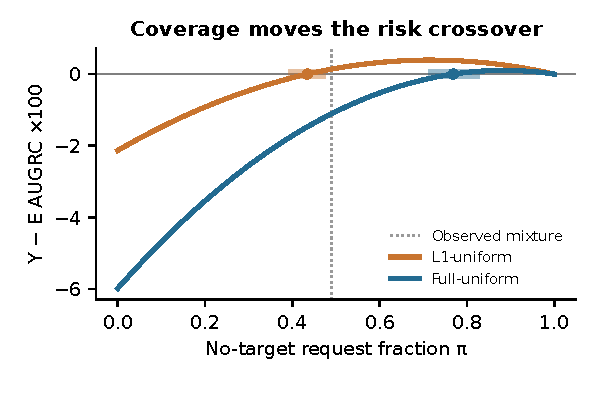
\includegraphics[width=\columnwidth]{generated/coverage_v8_r2/figure2_crossover.pdf}
\caption{\textbf{The tradeoff moves; it does not vanish.} FineCops Y$-$E
AUGRC under fixed class-conditional requests and varying no-target fraction.
Curves use the estimated mean pairwise AUROCs, not a fitted deployment rule.
Horizontal marks at zero show bootstrap intervals for the crossover location,
not confidence bands for the curves.}
\label{fig:crossover}
\end{figure}
\paragraph{Full coverage does not eliminate every residual loss.}
Y still trails E in FineCops C/N by $2.327$ $[1.730,2.948]$ points under
Full supervision. Its larger C/W advantage makes it preferable at the
observed mixture, but the relative risk can reverse when no-target requests
dominate. The internal crossover moves from $\pi=0.434$ $[0.401,0.467]$
under L1-uniform to $0.769$ $[0.721,0.819]$ under Full-uniform
(Fig.~\ref{fig:crossover}). Coverage changes the range of mixtures favoring
each target, rather than proving that the two learned abilities are now
jointly optimized for every population. This identity applies to AUGRC;
AURC is evaluated separately.

\section{Transfer and Practical Consequences}
\paragraph{The coverage response persists with frozen heads.}
On gRef source-disjoint requests, Full supervision changes Y risk by
\CovGRDY{} and E risk by\CovGRDE{}; Full TestA/B gives\CovFullDY{}
and\CovFullDE{}, respectively. All seeds agree on these risk directions.
For Y, C/N improves by 1.483 points while C/W decreases by 0.657 on the
source-disjoint surface, repeating the direction of the source-side tradeoff
with a smaller correctness cost. Both success comparisons deteriorate for E
there, even though its mean existence AUROC increases slightly.

Full-coverage Y$-$E C/N is unresolved on gRef source-disjoint
($+0.193$ $[-0.373,+0.777]$), whereas Y's C/W advantage is clear.
We therefore report improved complete risk without claiming pairwise
dominance. The two gRef surfaces overlap; they provide a source-exclusion
sensitivity, not two independent replications. Coverage training was
performed only on MM-GDINO. MDETR broadens the target/readout comparison,
not the coverage intervention's architecture scope.

\paragraph{Fixed score combinations offer setting-specific gains.}
An alternative practical response is to combine already learned scores.
On the original paired-L1 heads, we evaluate Product,
$\log\max(s_0,10^{-6})+\log\sigma(c_{G,E})$, and a prespecified SIRC-style
rule \cite{xia2024sirc}. Neither changes Native boxes; the latter uses
only training-positive normalization statistics. Product improves MM-GDINO
gRef source-disjoint AUGRC over Native, G/E and G/Y, including $-0.130$
$[-0.187,-0.074]$ relative to G/Y. On FineCops it is worse than both
learned heads. MDETR similarly shows reference- and population-dependent
gains. Full tables are in the supplement. These controls demonstrate that
fixed scores can sometimes be combined profitably, not a new fusion method
or dominance over the newly trained full-coverage heads.

\section{Discussion and Conclusion}
The central result is not that correct-output supervision is inherently
conflicted, or that one readout repairs confidence. Its effect depends on
the positive population used to learn it. With a fixed grounder and fixed
budget, expanding that population improves the Y head but worsens the E
head, changing the preferred target. The three-state decomposition explains
this response through a concrete exchange between C/W and C/N ordering,
and frozen transfer preserves the main risk directions.

For confidence design, this suggests an actionable sequence: specify the
event to be trusted, make the positive supervision population explicit,
and examine both success/failure comparisons before concluding that a
validity gain improves grounding reliability. Our intervention changes
positive examples, images and relative difficulty weights together; it is
not an isolated causal effect of a difficulty label. The evidence covers
two fixed localizers, with coverage intervention on one, three head seeds,
and text-negative/single-no-target requests. Within that scope, it advances
from observing different scores to identifying a training-population change
that alters their error priorities and downstream risk.

\FloatBarrier
{\small\bibliographystyle{ieeenat_fullname}\bibliography{references_empirical_v6}}
\end{document}
